\section{Μονοφασικός Αντιστροφέας Γέφυρας με μονοπολική PWM}
Μοντελοποιήθηκε ένας μονοφασικός αντιστροφέας γέφυρας με μονοπολική PWM τάσης εισόδου 100V και συχνότητα 50Hz στο οποίο εφαρμόζεται το ίδιο RL φορτίο (R = 10Ω, L = 0.025Η). Για την καλύτερη κατανόηση του, προσομοιώθηκε η λειτουργία του για $m_a = 0.9$ και $m_f = 40$  και $m_f = 200$ και καταγράφηκαν οι ακόλουθες κυματομορφές.

\subsection{Κυματομορφές Κυκλώματος}

\subsubsection*{Τάση και Ρεύμα εξόδου}
\begin{figure}[h!]
	\begin{subfigure}{0.49\textwidth}
		\centering
		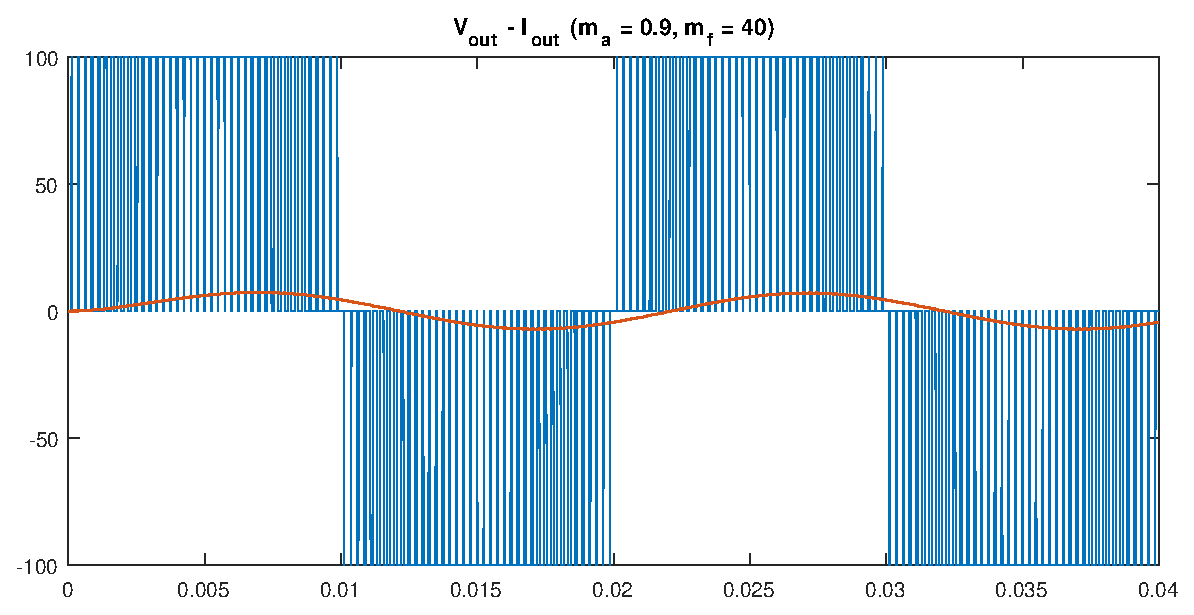
\includegraphics[width=1\textwidth]{Images/V_out_I_out_40}
	\end{subfigure}
	\begin{subfigure}{0.49\textwidth}
		\centering
		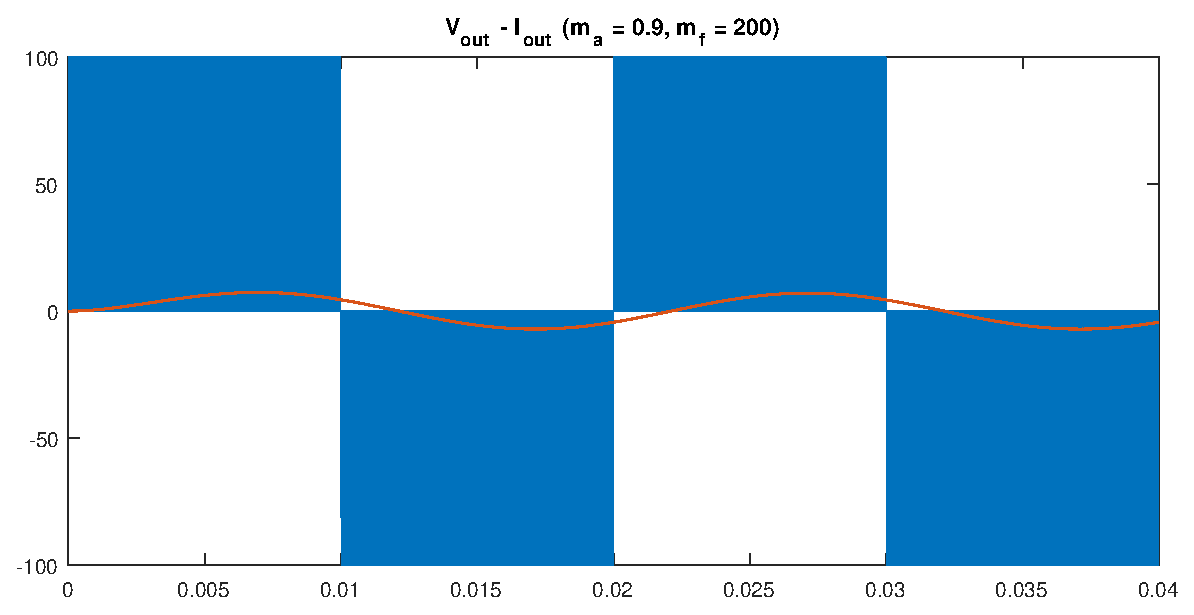
\includegraphics[width=1\textwidth]{Images/V_out_I_out_200}
	\end{subfigure}
	\noindent
	Σύμφωνα με τα παραπάνω figures, τόσο η τάση όσο και το ρεύμα εξόδου έχουν την αναμενόμενη μορφή, όπου το σήμα της τάσης αποτελείται από διακριτούς παλμούς και το ρεύμα εξόδου παρουσιάζει ημιτονοειδή μορφή.
	\subsubsection*{Τάση εξόδου}
	\begin{subfigure}{0.49\textwidth}
		\centering
		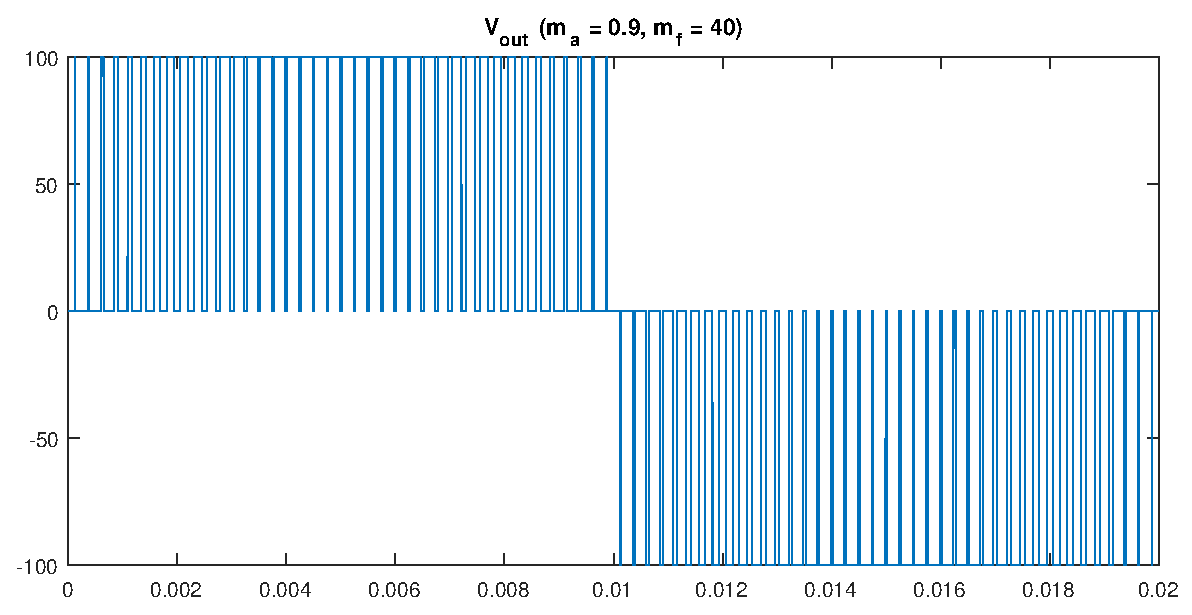
\includegraphics[width=1\textwidth]{Images/V_out_40}
	\end{subfigure}
	\begin{subfigure}{0.49\textwidth}
		\centering
		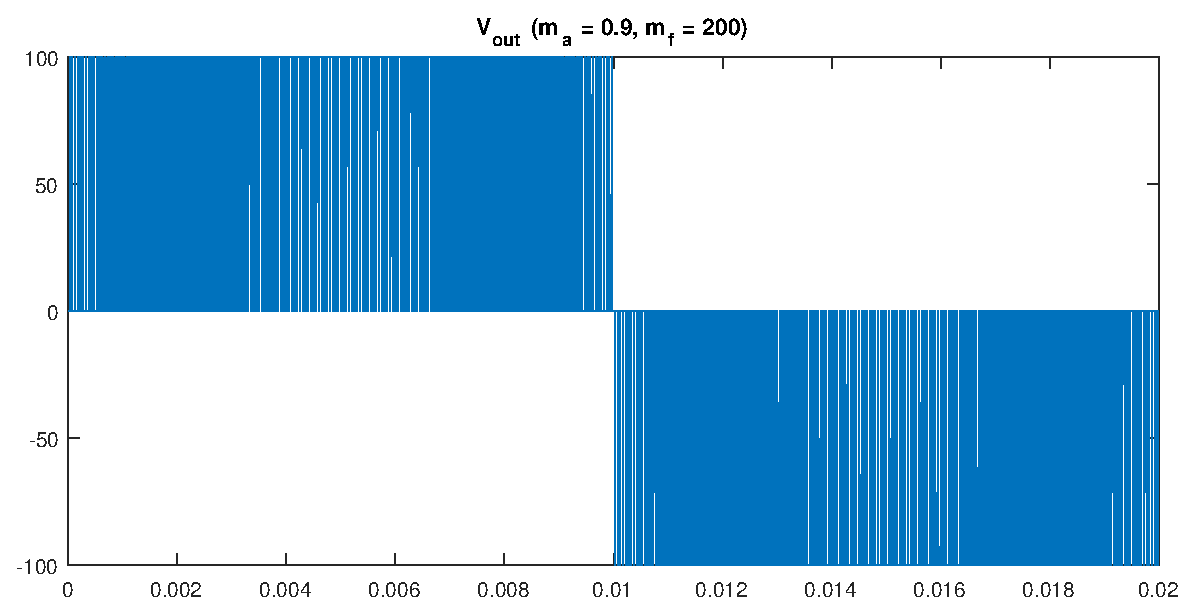
\includegraphics[width=1\textwidth]{Images/V_out_200}
	\end{subfigure}
\end{figure}
\noindent
Όσον αφορά την τάση εξόδου, αυξάνοντας τον $m_f$ παρατηρείται αύξηση του αριθμού των παλμών τάσης, συμπεριφορά  η οποία ήταν αναμενόμενη καθώς όπως προαναφέρθηκε στην υποενότητα \ref{single_PWM}, αυξάνοντας τον $m_f$ αυξάνεται ανάλογα η συχνότητα του τριγωνικού παλμού. Η αύξηση αυτή σε συνδυασμό με την σταθερή συχνότητα του επιθυμητού ημιτόνου, οδηγεί σε αύξηση των παλμών τάσης εφόσον αυτοί προκύπτουν μέσω σύγκρισης των δύο σημάτων.\\

\begin{figure}[h!]
	\subsubsection*{Ρεύμα εξόδου}
	\begin{subfigure}{0.49\textwidth}
		\centering
		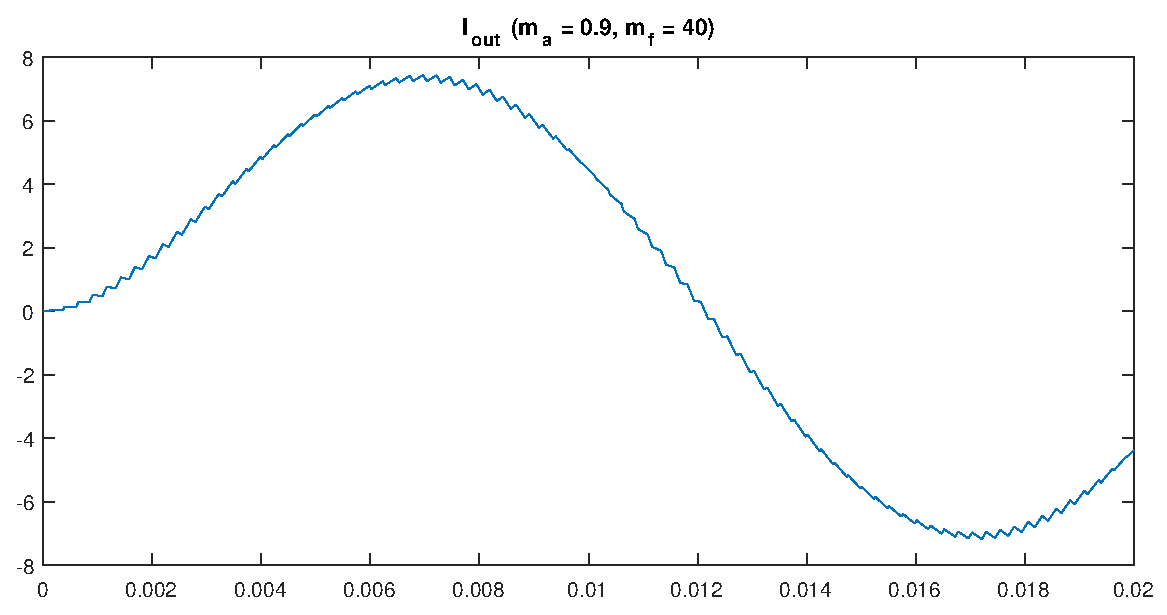
\includegraphics[width=1\textwidth]{Images/I_out_40}
	\end{subfigure}
	\begin{subfigure}{0.49\textwidth}
		\centering
		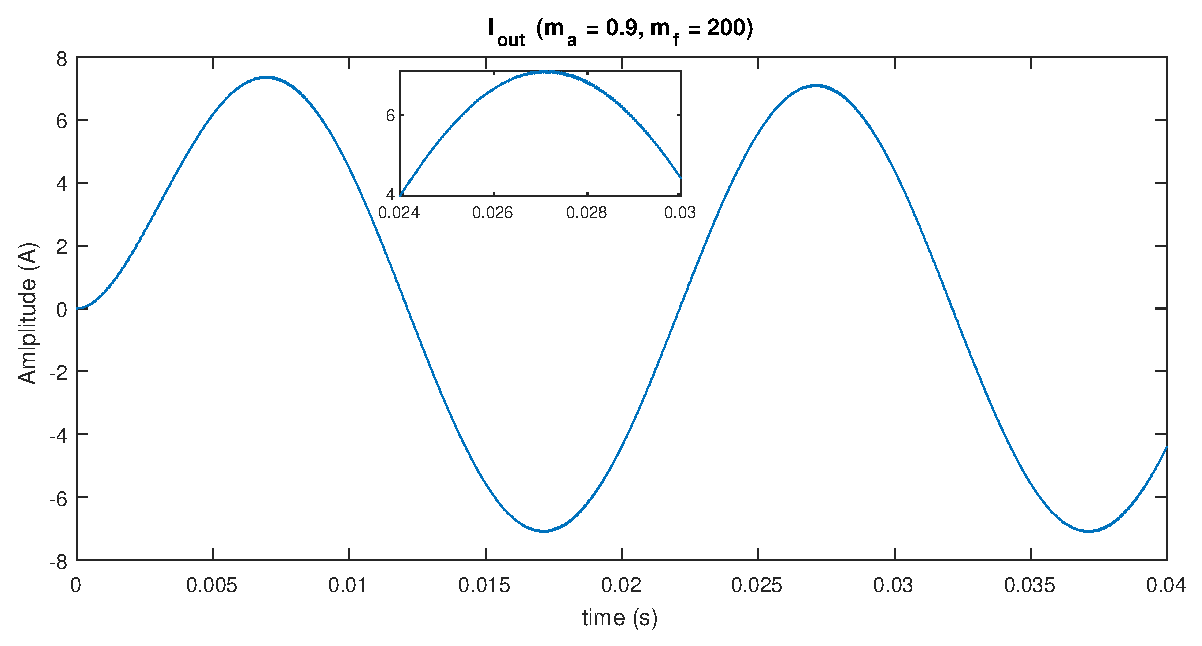
\includegraphics[width=1\textwidth]{Images/I_out_200}
	\end{subfigure}
\end{figure}
\noindent
Όσον αφορά το ρεύμα εξόδου, αυξάνοντας το $m_f$ παρατηρείται μείωση των διακυμάνσεων η οποία συνεπάγεται με μείωση των αρμονικών στο σήμα.
Η μείωση αυτή οφείλεται εν μέρη στο γεγονός πως το φορτίο είναι ωμικοεπαγωγικό και όπως είναι γνωστό, η σύνθετη αντίσταση του ισούται με $R + j\omega L$, οπότε αυξάνοντας τον $m_f$, αυξάνοντας πρακτικά την συχνότητα του φέροντος, αυξάνεται και η σύνθετη αντίσταση του μειώνοντας  έτσι την επίδραση των ανώτερων αρμονικών.

\noindent\\
 Ακόμη όπως προαναφέρθηκε (υποενότητα \ref{single_PWM}), αυξάνοντας τον $m_f$ οι αρμονικές του σήματος εμφανίζονται σε μεγαλύτερες συχνότητες με αποτέλεσμα να έχουν μικρότερη επιρροή.\\

\begin{figure}[h!]
	\subsubsection*{Τάση Transistor}
		\begin{subfigure}{0.49\textwidth}
		\centering
		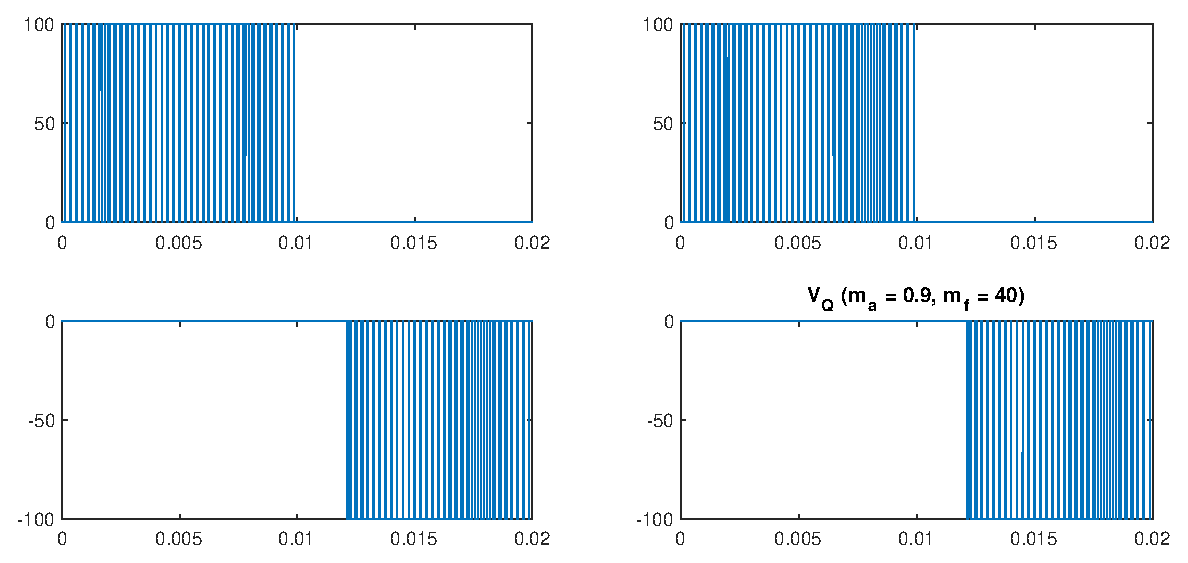
\includegraphics[width=0.95\textwidth]{Images/V_Q_40}
	\end{subfigure}
	\begin{subfigure}{0.49\textwidth}
		\centering
		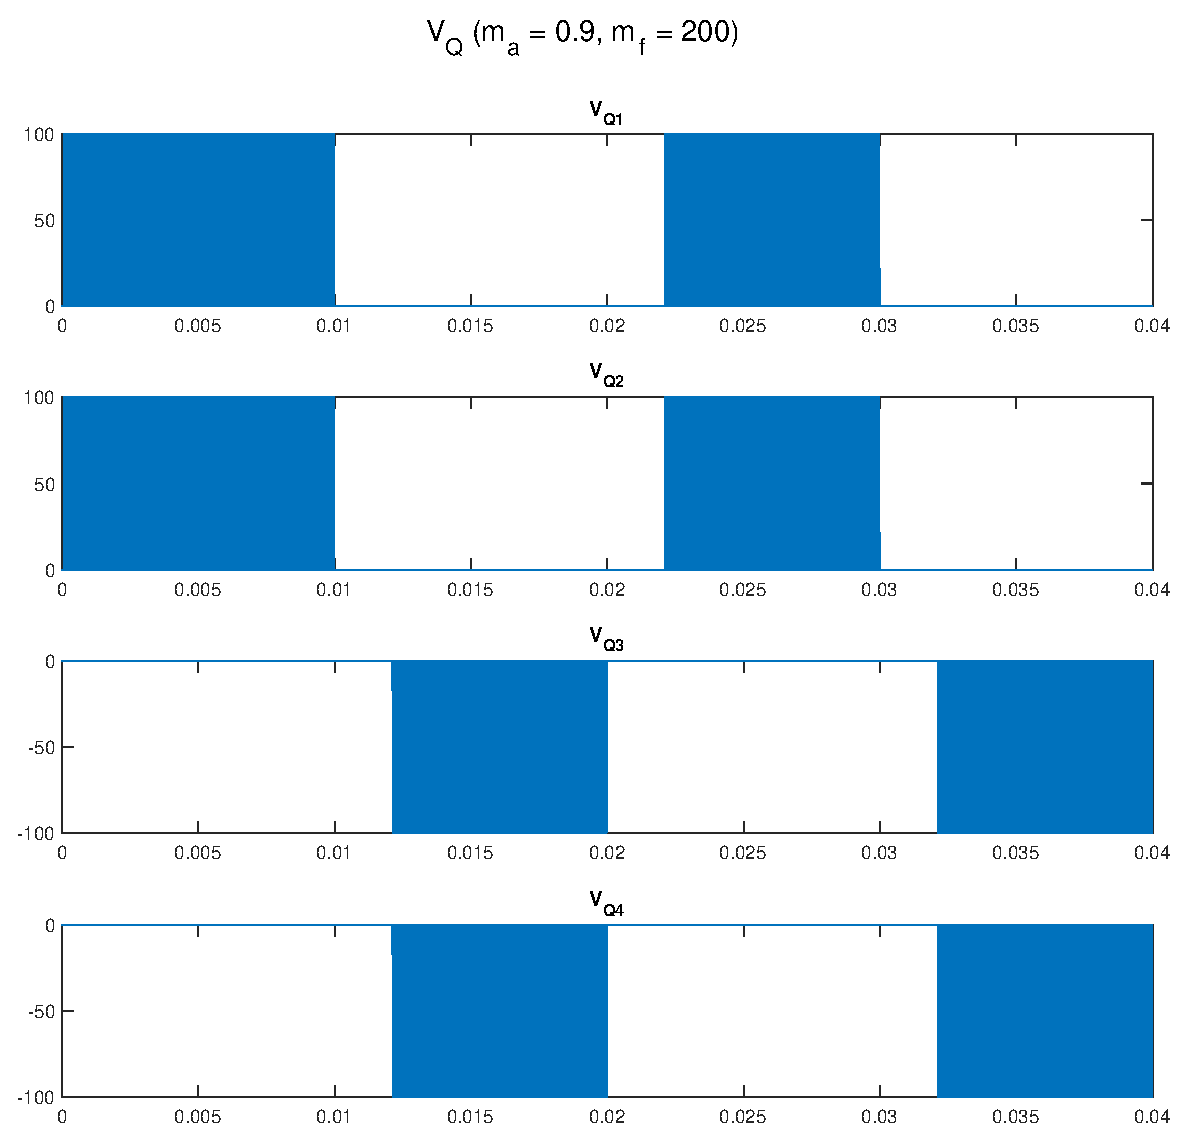
\includegraphics[width=0.95\textwidth]{Images/V_Q_200}
	\end{subfigure}
\end{figure}
\noindent
Όσον αφορά την τάση στα transistor, παρατηρείται πως τα transistor άγουν σε ζεύγη (1-2 και 3-4) σύμφωνα με την υποενότητα \ref{} καθώς και πως αποτελείται από παλμούς διαφορετικού εύρους.  Ακόμα, σε σχέση με τον \textbf{Μετατροπέα Quasi}, οι παλμοί έχουν τό ίδιο πλάτος τις αντίστοιχες χρονικές στιγμές καθώς προκύπτουν ακολουθώντας την ίδια διαδικασία. Τέλος, αυξάνοντας τον $m_f$ παρατηρείται και πάλι πενταπλασιασμός των παλμών.\\
\begin{figure}[h!]
	\subsubsection*{Ρεύμα Transistor}
	\begin{subfigure}{0.49\textwidth}
		\centering
		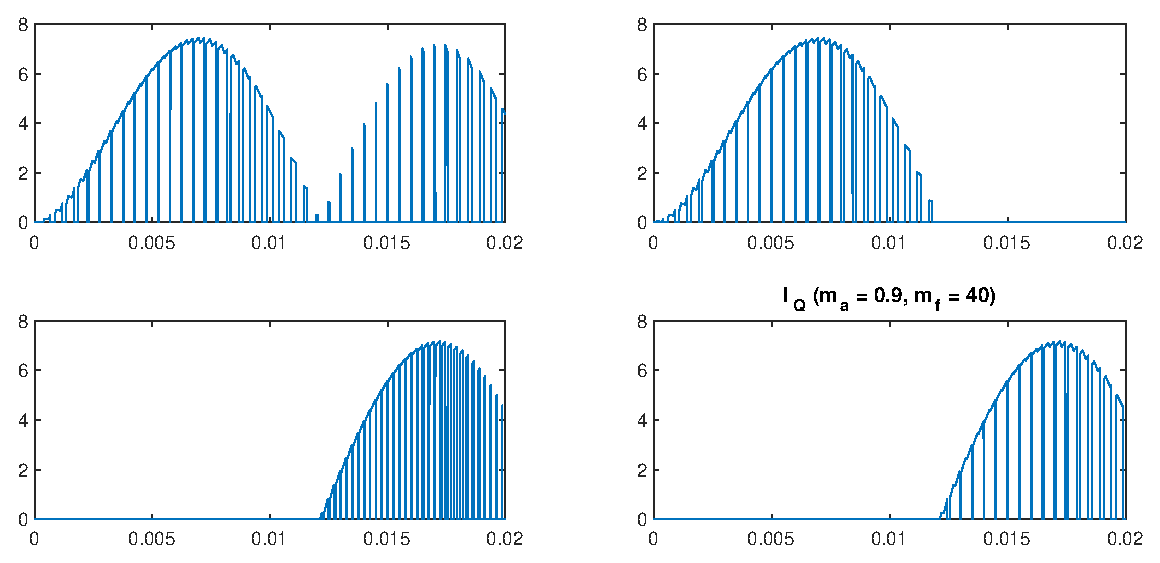
\includegraphics[width=0.95\textwidth]{Images/I_Q_40}
	\end{subfigure}
	\begin{subfigure}{0.49\textwidth}
		\centering
		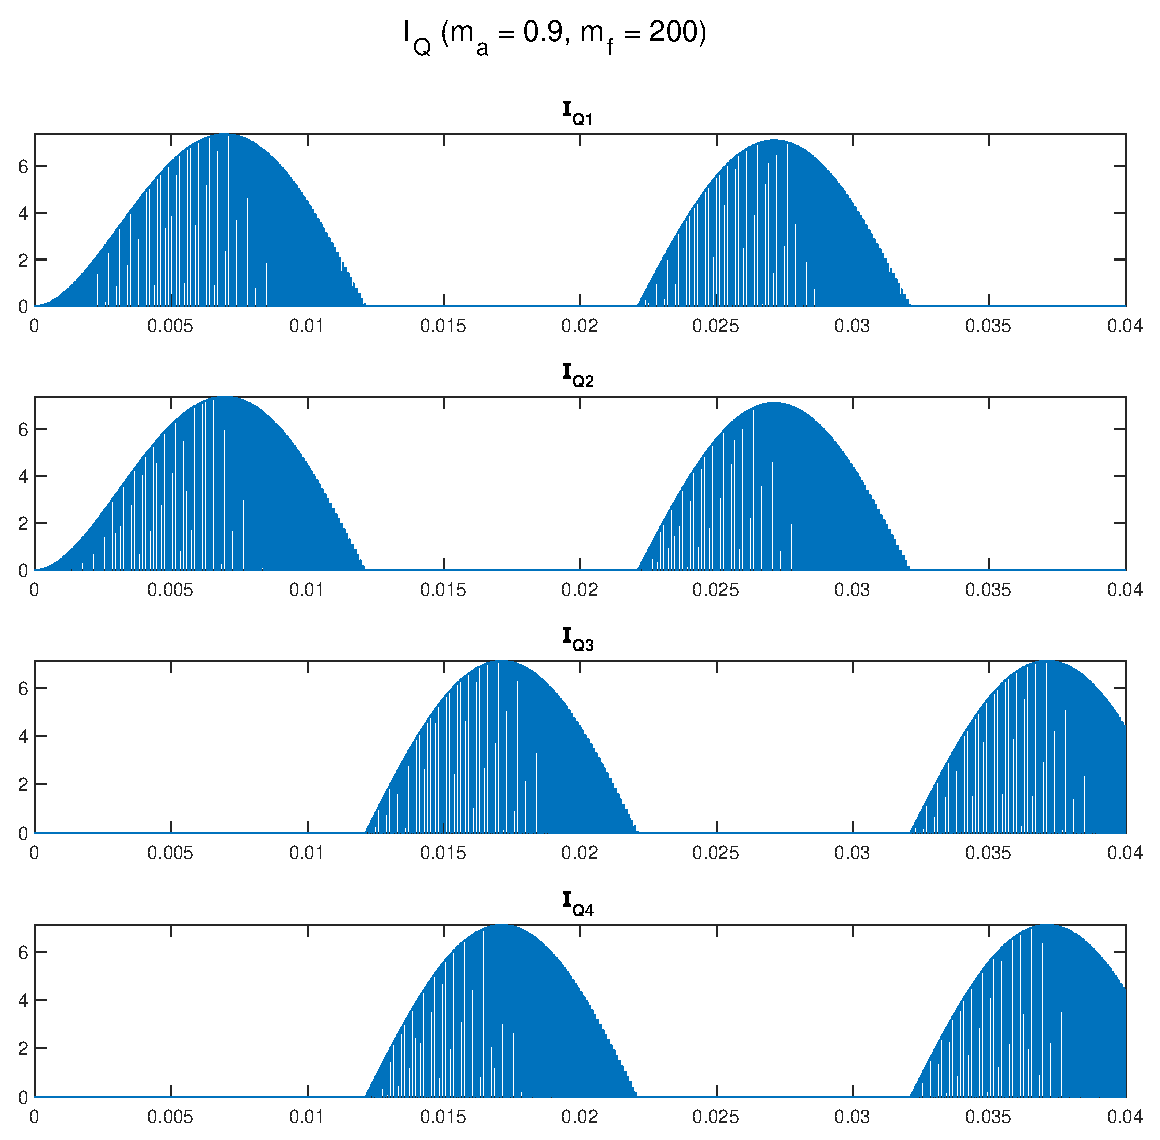
\includegraphics[width=0.95\textwidth]{Images/I_Q_200}
	\end{subfigure}
	\noindent
	Παρατηρώντας τις κυματομορφές ρεύματος των transistor είναι και πάλι εμφανές πως άγουν σε ζεύγη καθώς και πως για πενταπλασιασμό του $m_f$ πενταπλασιάζονται οι παλμοί.\textbf{Ισως πως οτι ειναι πιο sm}
\end{figure}

\begin{figure}[h!]
	\subsubsection*{Τάση Διόδων}
	\begin{subfigure}{0.49\textwidth}
		\centering
		\includegraphics[width=0.95\textwidth]{Images/V_D_40}
	\end{subfigure}
	\begin{subfigure}{0.49\textwidth}
		\centering
		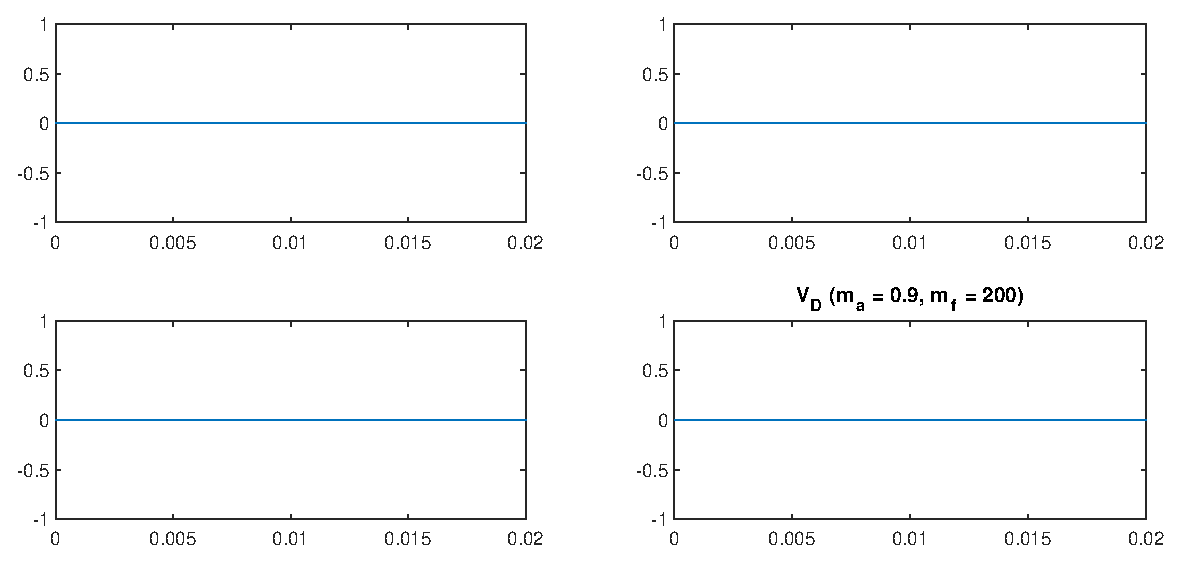
\includegraphics[width=0.95\textwidth]{Images/V_D_200}
	\end{subfigure}
	\noindent
	Ομοίως με τον \textbf{Quasi wave}, η τάση των διόδων είναι ίση με 0 καθώς όπως προαναφέρθηκε, άγουν μόνο στις περιπτώσεις όπου η τάση εξόδου είναι ίση με 0?!!?!?!?!?!?!??! 
\end{figure}

\begin{figure}[h!]
	\subsubsection*{Ρεύμα Διόδων}
	\begin{subfigure}{0.49\textwidth}
		\centering
		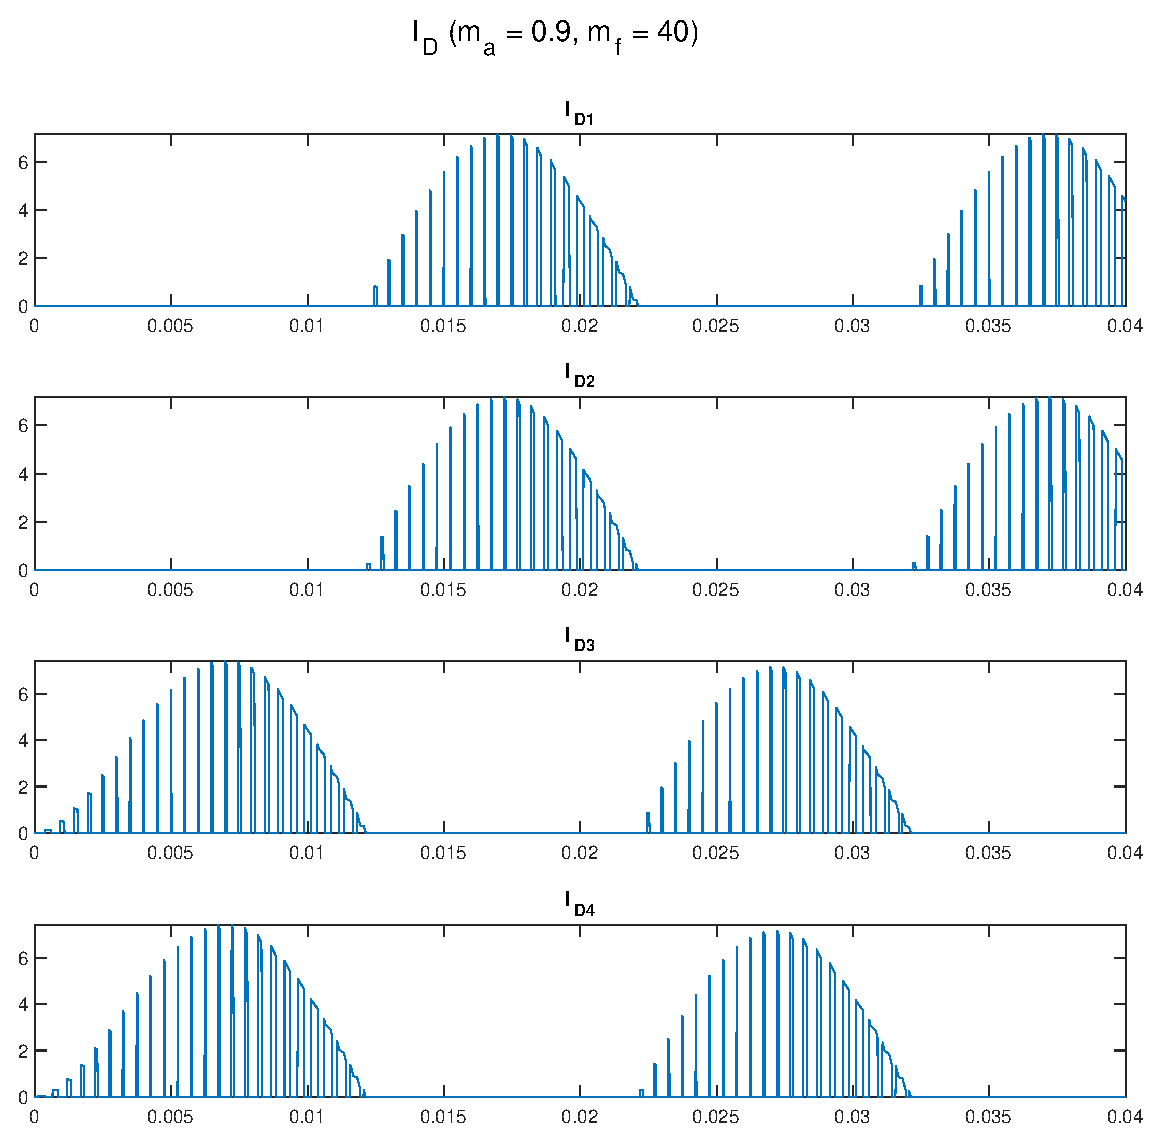
\includegraphics[width=0.95\textwidth]{Images/I_D_40}
	\end{subfigure}
	\begin{subfigure}{0.49\textwidth}
		\centering
		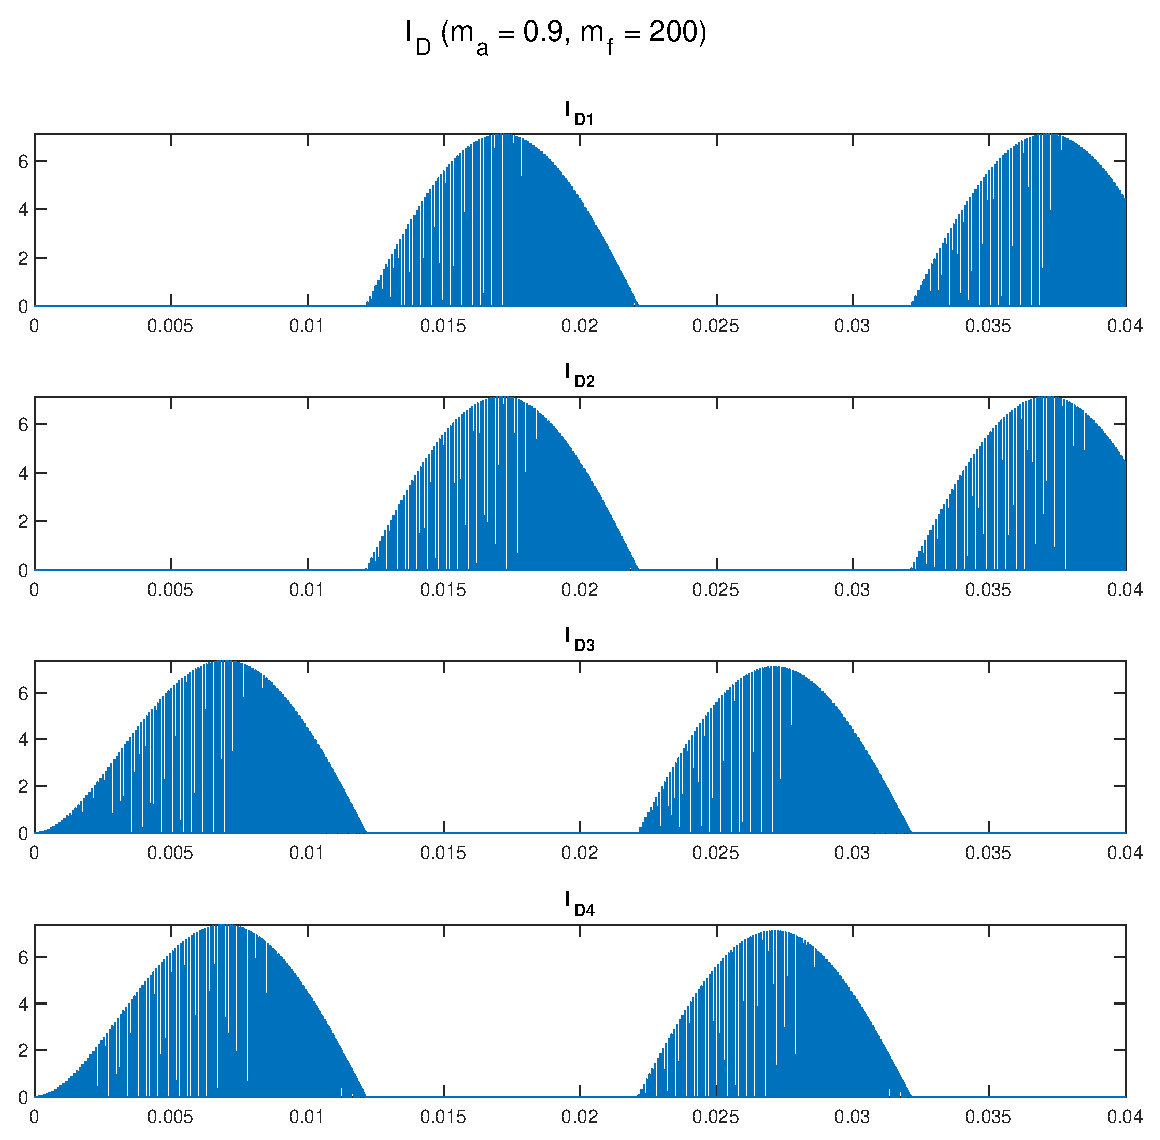
\includegraphics[width=0.95\textwidth]{Images/I_D_200}
	\end{subfigure}
\end{figure}
\noindent
Σε αντίθεση με την τάση των διόδων, το ρεύμα δεν είναι μηδενικό αλλά παρουσιάζει όμοια μορφή με το ρεύμα των transistor, με βασική διαφορά πως μπορεί να ρέει ρεύμα μόνο μέσω της αντίστοιχης διόδου ή του αντίστοιχου transistor.

\subsubsection*{Ισχύς Εισόδου - Εξόδου}
Για τον υπολογισμό της ισχύς απαιτείται γνώση του ρεύματος. Όσον αφορά την έξοδο του κυκλώματος, το ρεύμα είναι γνωστό ωστόσο όσον αφορά την είσοδο, το ρεύμα είναι απαραίτητο να βρεθεί. 

\noindent\\
Εφαρμόζοντας νόμο ρευμάτων του Kirchhoff, προκύπτει η εξής σχέση για το ρεύμα εισόδου $I_{in}$:
\begin{equation}
	I_{in} - I_{Q_1} + I_{D_1} - I_{Q_3} + I_{D_3} = 0 \xRightarrow{} I_{in} = I_{Q_1} - I_{D_1} + I_{Q_3} - I_{D_3} 	
\end{equation}

οπότε εφόσον η ισχύς υπολογίζεται ως το γινόμενο μεταξύ τάσης και ρεύματος, οι ισχύς προκύπτουν ως εξής:
\begin{align}
	P_{in} &= V_{in} \cdot I_{in} = V_{dc} \cdot I_{in}\\
	P_{in} &= V_{out} \cdot I_{out}
\end{align}

\subsection{Συντελεστής Ισχύος}